\chapter{Introduction}

\textit{The introduction provides a thorough review of the background, including relevant literature, the motivation, the aims of the thesis and the hypotheses. Literature references for the thesis should be collected in one common bibliography at the end of the thesis.}


\section{Medical Motivation}

\subsection{Anatomy}

\begin{figure}[htbp]
    \begin{minipage}[c][0.9\textheight][t]{.5\textwidth}
        \centering
        \vspace*{\fill}
        \subfloat[The PNS of the upper extremity.]
        {
            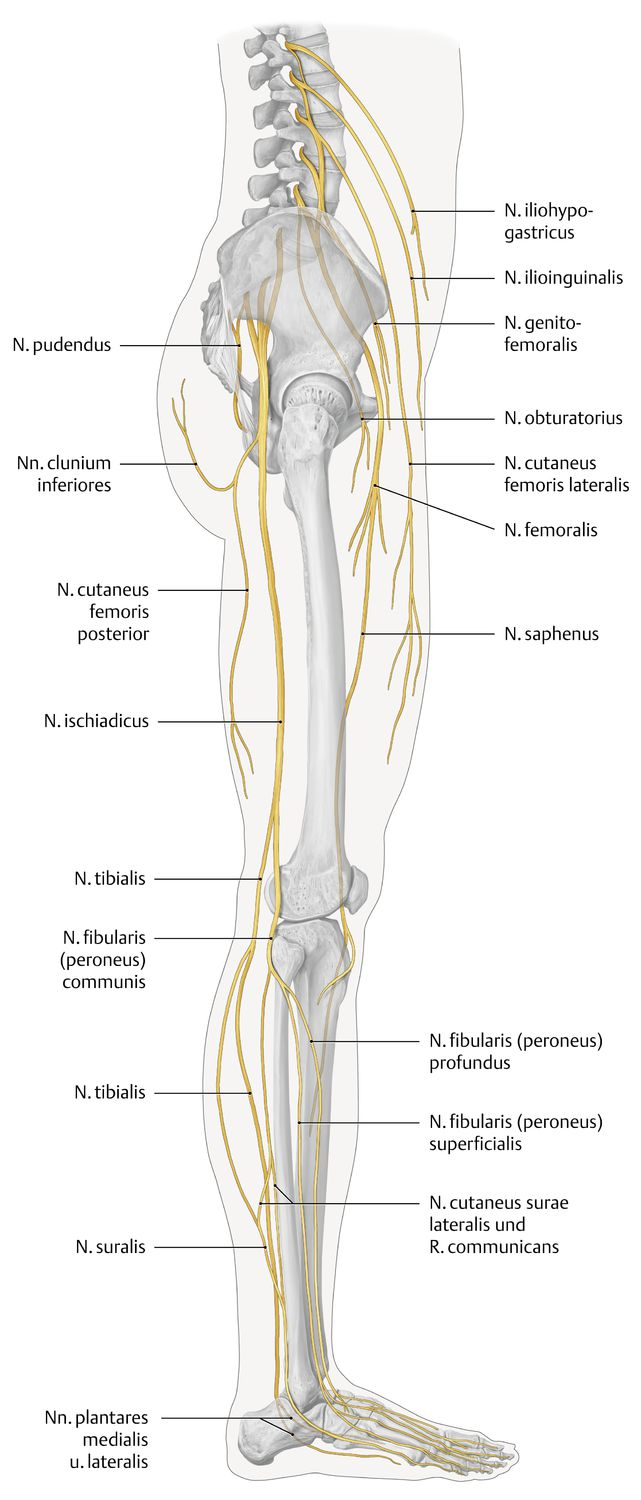
\includegraphics[width=\linewidth]{anat_sagittal}
            \label{fig:subfig:anat_sagittal}
        }
    \end{minipage}
    \begin{minipage}[c][0.9\textheight][t]{.5\textwidth}
        \centering
        \vspace*{\fill}
        \subfloat[Cross-section of the right upper arm (proximal view).]
        {
            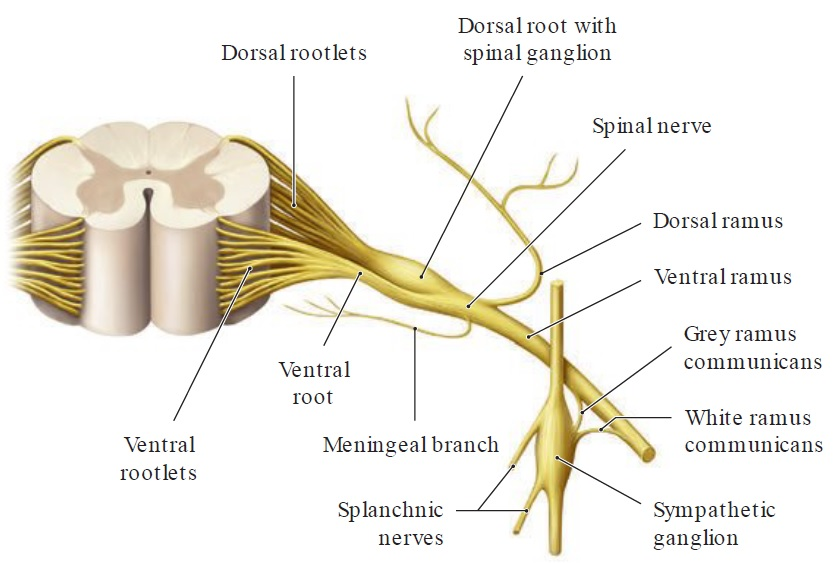
\includegraphics[width=\linewidth]{anat_spinal}
            \label{fig:subfig:anat_spinal}
        }
        \vfill
        \subfloat[Cross-section of the right lower arm (proximal view).]
        {
            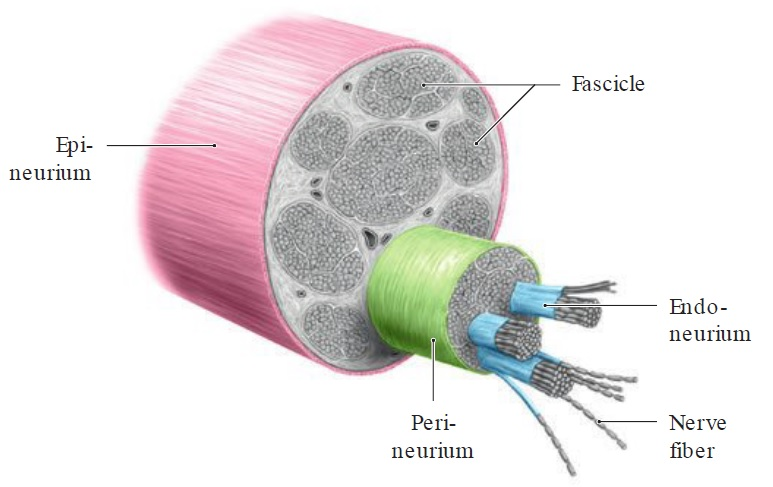
\includegraphics[width=\linewidth]{anat_nerve}
            \label{fig:subfig:anat_nerve}
        }
    \end{minipage}
    \vspace*{-0.3cm}
    \caption[Anatomy of the Peripheral Nervous System of the Lower Extremity]{\textbf{a)} Figure~C p.~537 from~\cite{Schunke2014PrometheusAnatomie}. \textbf{b)} Figure~B p. 384 and \textbf{c)} Figure~D p. 265 from~\cite{Schunke2015THIEMEAnatomy}.}
    \label{fig:anat}
\end{figure}

\begin{figure}[htbp]
	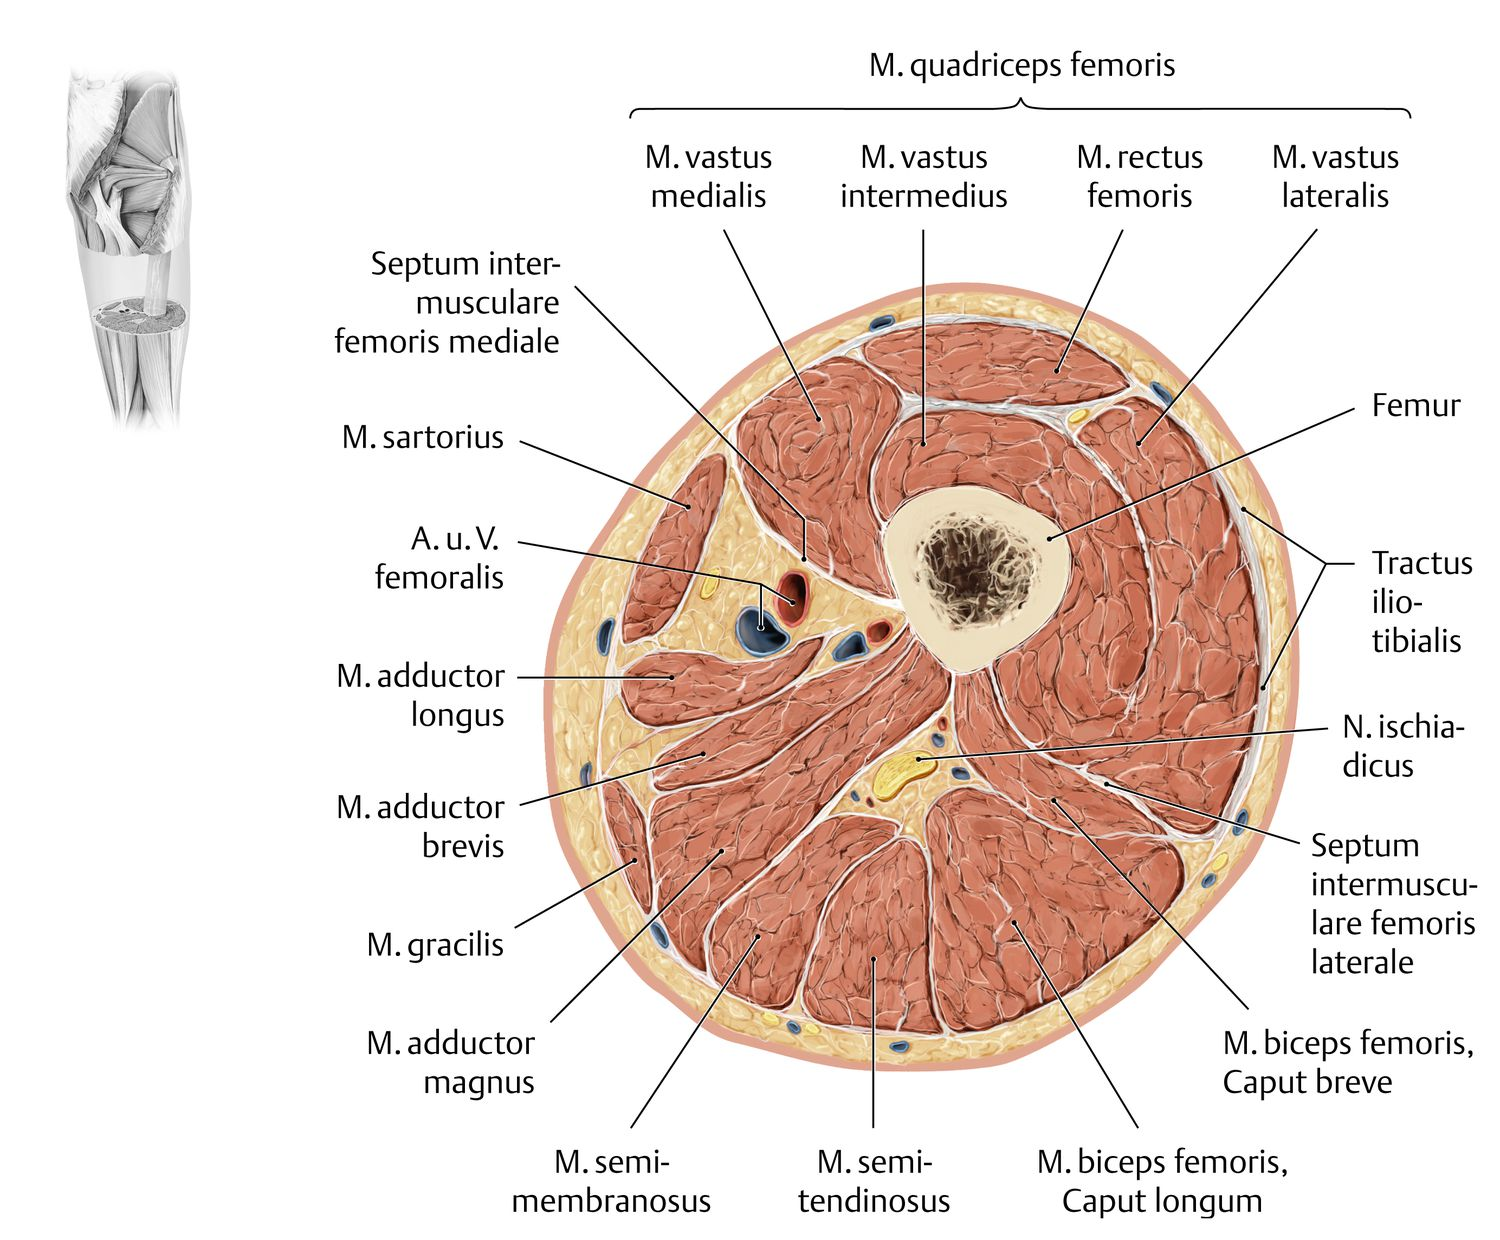
\includegraphics[width=\textwidth]{anat_axial}
    \caption[Cross-section of the Right Upper Leg]{Figure~A p. 528 from~\cite{Schunke2014PrometheusAnatomie}}
    \label{fig:anat_axial}
\end{figure}


\subsection{Peripheral Neuropathies}

\subsection{State-of-the-Art Diagnosis}

\section{Medical Image Segmentation}

\section{Machine Learning}
In this part we brielfy describe some fundamentals for machine learning. Section~\ref{sec:ml_supervised} introduces the topic of supervised learning on an example.

\subsection{Supervised Learning} \label{sec:ml_supervised}
The principle of supervised learning is illustrated on the prediction of house prizes as a function of their living area in Figure~\ref{fig:dl_supervised} taken from~\cite{Ng2012StanfordNotes}. In supervised learning, we train an algorithm (or also called model) by showing the algorithm input-output pairs (e.g., living area of houses versus their corresponding prizes). This is referred to as the training phase, and the input-output pairs are called the training set. The outputs are typically referred to as labels or targets. More formally we define the training set as
\begin{equation}
   S_{Train} = \{(x^{(i)}, y^{(i)}); i = 1,...,m\}
   \label{eq:training_set}
\end{equation}
and let $\chi$ and $\upsilon$ denote the space of input and output values, respectively. In this example, $\chi = \upsilon = \mathbb{R}$. The aim of the training phase is to let the algorithm (hopefully) learn a meaningful relationship between the inputs and outputs of our training set. Therefore, we aim learn a mapping $h : \chi \mapsto \upsilon$, parameterized by a set of models weights~$\textbf{W}$, which is "good" for all pairs in $S_{Train}$, hence
\begin{equation}
   y^{(i)} = h(x^{(i)}, \mathbf{W}); i = 1,...,m
   \label{eq:model}
\end{equation}
is approximatively valid for all training pair. We call $h(x^{(i)}, \mathbf{W})$ our model with the model weights~$\textbf{W}$. Depending on the on the type of mapping, $\mathbf{W}$ is typically a Matrix and we therefore, write it in bold font. If the learned relation is correct, the model can be used to make predictions on previously unseen input data.\\
If the output, we are trying to predict, is continuous, such as in the housing example, the problem is called a \textbf{regression problem}. We could also have the case where we wanted to predict whether the dwelling is an apartment or a house, given the living area. The predicted output would, therefore, be discrete and we would call this a \textbf{classification problem}.\\
Supervised learning gets its name for the reason that the algorithm always learns on input-output pairs (the outputs typically called labels or targets), and the outputs typically are the result of (laborsome) labeling work done by a person. This is the biggest drawback of supervised learning. There, however, exist ways to use unlabeled data in conjunction with labeled data, referred to as semi-supervised learning. Learning on inputs only corresponds to finding patterns and structures in the input space and is referred to as unsupervised learning. Typical examples for unsupervised learning algorithms are \gls{pca} and $k$-means Clustering~\cite{Goodfellow2016DeepLearning}.\\
For the presented example, one could expect a linear relationship, between the living area of a house and its prize. If this was indeed true, we could make robust predictions with a simple linear model, i.e. $y^{(i)} = h(x^{(i)}, W) = Wx^{(i)} + b$, only incorporating the living area. However, one could argue that the number of rooms or the location, each with its unknown weight, also influence the dwelling's prize. These influencers are typically called features. There was, and still, is a whole science around finding good features to solve learning problems.\\
This is precisely what F. Balsiger did during his master thesis~\cite{Balsiger2016DevelopmentApproaches}: He investigated the different impact features had on the segmentation results of the peripheral nerves done by a trained \gls{rf}~\cite{Breiman2001RandomForests}. The \gls{rf}, also belonging to supervised learning, was trained by engineered features calculated on the \gls{mrn} images. This resulted in a voxel-wise classification into the labels \textit{peripheral nerve} and \textit{background}, hence a segmentation of the peripheral nerves. \\
The main drawback of any learning algorithm relying on features is, however, that the algorithm is inherently constrained by the imagination and ability of the engineer to find and implement good features.

\begin{figure}[htbp]
    \centering
	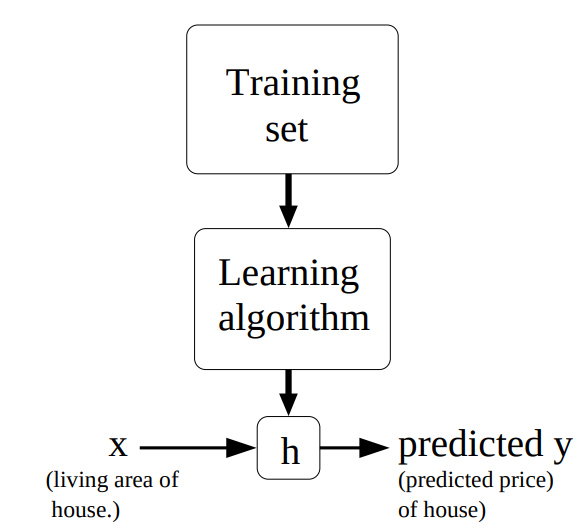
\includegraphics[width=0.5\textwidth]{supervised_learning}
    \caption[Supervised Learning]{The principle of supervised learning illustrated on the example of predicting house prices (y) depending on the living area (x). Suppose we have $m$ area-price pairs, which we name our training set: $\{(x^{(i)}, y^{(i)}); i = 1,...,m\}$. We let $\chi$ and $\upsilon$ denote the space of input and output values, respectively. In this example, $\chi = \upsilon = \mathbb{R}$. In supervised learning we aim to learn a function (also called mapping) $h : \chi \mapsto \upsilon$, which makes reasonable prize prediction (y) for a given new house area (x). We use the training set to learn $h$. Image and example taken from~\cite{Ng2012StanfordNotes}.}
    \label{fig:dl_supervised}
\end{figure}

\subsection{Training}
In the previous section we defined that the model $h(x^{(i)}, \mathbf{W})$ is parameterized by the set of weights $\textbf{W}$. During the training phase of the model, we adjust $\textbf{W}$ in order for the model to make "better" predictions on the training set. Formally, we want to solve the optimization problem
\begin{equation}
   \mathbf{W}^{*} = \argmin_\textbf{W} \sum_{i=1}^{m} L(h(x^{(i)}, \mathbf{W}), y^{(i)})
   \label{eq:optimization}
\end{equation}
where $L(...)$ denotes a loss function. The loss function is a metric we have to choose, which calculates the error between the correct label $y^{(i)}$ and the prediction our model made. The loss function is often also referred to as cost function. $\mathbf{W}^{*}$ denotes the solution for the mentioned optimization problem and, consequently, is the set of weights which results in the smallest error in our training set. Training of a model corresponds to iteratively decreasing the training error.\\
A loss function typically used for classification problems with $k$ classes, a prediction vector $\mathbf{h}^{(i)}$ and label vector $\mathbf{y}^{(i)}$, is the cross-entropy loss

\begin{equation}
    L(\mathbf{h}^{(i)}, \mathbf{y}^{(i)}) = -\mathbf{y}^{(i)} \log(f(\mathbf{h}^{(i)}))
    \label{eq:cross_entropy_multi}
\end{equation}
with $f(...)$ being the softmax activation function
\begin{equation}
   f(\mathbf{h}^{(i)}) = \frac{\exp\mathbf{h}^{(i)}}{\sum_{j} \exp{\mathbf{h}^{(i)}_{j}}}
   \label{eq:softmax}
\end{equation}
which squashes the predictions into a vector of values between zero and one that add up to one. The corresponding cross-entropy loss for a binary classification problem
\begin{equation}
    L({h}^{(i)}, {y}^{(i)}) = -{y}^{(i)} \log(\sigma({h}^{(i)}))
    \label{eq:cross_entropy_binary}
\end{equation}
with $\sigma(...)$ being the sigmoid activation function
\begin{equation}
   \sigma({h}^{(i)}) = \frac{1}{1 + \exp{(-{h}^{(i)})}}
   \label{eq:sigmoid}
\end{equation}
Another, in deep learning very popular, activation function is the \gls{relu}, defined as
\begin{equation}
   ReLU({h}^{(i)}) = \max(0, {h}^{(i)})
   \label{eq:relu}
\end{equation}

In order to solve Equation~\ref{eq:optimization}, optimizer are used. Optimizer, such as \gls{sgd}~\cite{Goodfellow2016DeepLearning} and Adam~\cite{Kingma2014Adam:Optimization} use the gradient to find $\textbf{W}^*$. The gradient depends on the model and the chosen loss function and corresponds the first order derivative of the individual inputs with respect to the output.\\

A common problem in machine learning, especially in deep learning, is the problem of under- and overfitting, which is depicted in Figure~\ref{fig:under_over_fitting}. To solve a learning problem, we have to choose a model first. The model's representational power, hence the ability to fit a wide variety of functions, is called capacity~\cite{Goodfellow2016DeepLearning}. If the models capacity is too low for the task at hand, it cannot model the relationship between the input and output. This is called underfitting. On the other hand, if the models capacity is too high, it can start to memorize the data it was trained upon (including the data's statistics) rather than learning structures or relationships. This results in a bad performance on new data, hence bad generalization and is called overfitting.

\begin{figure}[htbp]
    \centering
	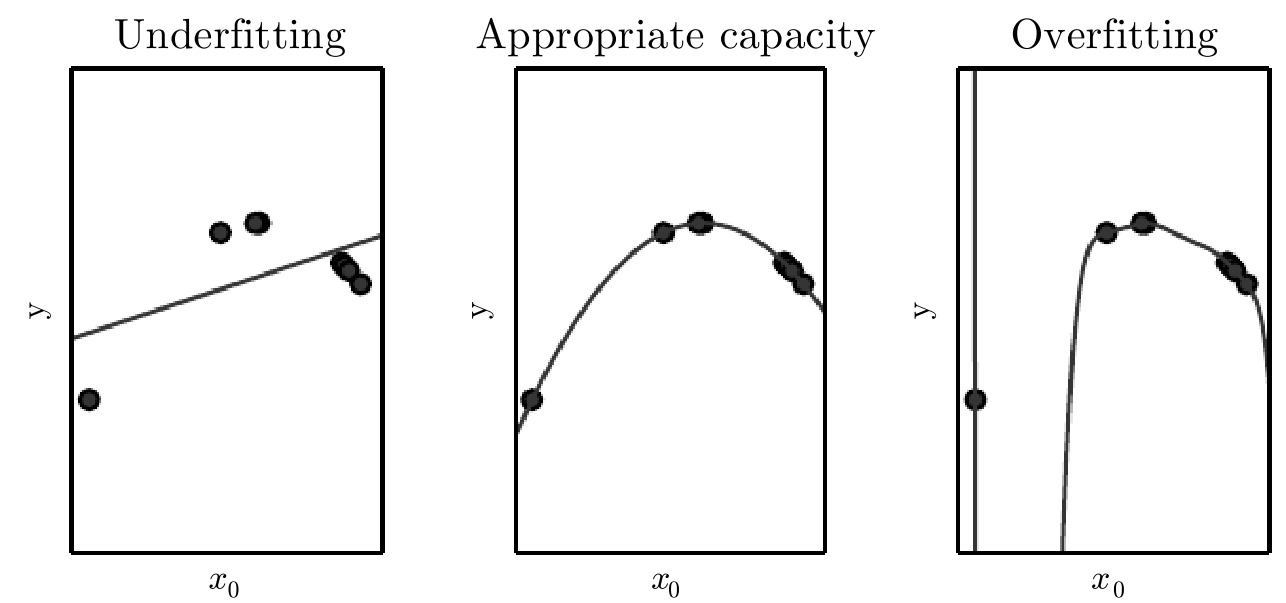
\includegraphics[width=0.8\textwidth]{under_over}
    \caption[Under- and Overfitting]{The problem of under- and overfitting. The sample points were generated by random sampling a quadratic function. In the left image, a model with low capacity (a line) is not able to correctly capture the structure of the points. The center image shows that a quadratic model would generalize well to unseen ponts. The right image shows that a 9\textsuperscript{th} degree polynomial perfectly catches all points but would generalize bad to new points. Image and example taken from~\cite{Goodfellow2016DeepLearning}.}
    \label{fig:under_over_fitting}
\end{figure}

\subsection{Deep Learning \& Convolutional Neural Networks}
With increasing amounts of labeled data, gathered in big datasets, and increasing computational performance using \gls{gpu}'s, the creation and training of models, called neural networks, with much larger capacity became possible. Today, some of the biggest datasets for images are ImageNet~\cite{Russakovsky2015ImageNetChallenge} and Microsoft's COCO~\cite{Lin2014MicrosoftContext}.
The most significant advantage of those models was that (given enough training data) it was now possible to train them directly on raw, unprocessed data, rather than on human-engineered features which may be suitable for a given task or not.
\gls{cnn}s, a class of neural network mostly used to analyze visual imagery, were successfully applied \cite{Lecun2015DeepLearning} achieved new levels of performances in computer vision tasks and challenges \cite{Krizhevsky2012ImageNetNetworks,Simonyan2014VeryRecognition}.

\subsection{Convolutional Neural Networks}
\cite{KarpathyStanfordRecognition}

\subsubsection{Convolutional Layer}
\subsubsection{Pooling Layer}
\subsubsection{Normalization Layer}
\subsubsection{Fully-Connected Layer}

\subsubsection{Visualizations}



\section{Related Work}
\section{Hypothesis}

\textit{Deep-learning-based segmentation of peripheral nerves from \gls{mrn} images is possible.} \\
\textit{3D-Contextual information allows for better segmentation results.}

\section{Aim \& Structure of the Thesis}

\endinput